\documentclass[conference]{IEEEtran}
\usepackage{cite}
\usepackage{amsmath,amssymb,amsfonts}
\usepackage{algorithmic}
\usepackage{graphicx}
\usepackage{textcomp}
\usepackage{xcolor}
\usepackage{tikz}
\usetikzlibrary{shapes.geometric, arrows}

\def\BibTeX{{\rm B\kern-.05em{\sc i\kern-.025em b}\kern-.08em
    T\kern-.1667em\lower.7ex\hbox{E}\kern-.125emX}}

\begin{document}

% ==================================================================
% TITLE
% ==================================================================
\title{Robust Electronic Nose System for Atmospheric Gas Classification using Normalized Kinetic Feature Extraction}

% ==================================================================
% AUTHORS (Alphabetical Order)
% ==================================================================
\author{\IEEEauthorblockN{Abhishek Srivastava, Alan Nelson, Bysani Vedavyas, Devshree Vyas, \\
Kushagra Agrawal, Shreyas Agarwal, Srikar Somanchi}
\IEEEauthorblockA{\textit{International Institute of Information Technology Hyderabad} \\
Hyderabad, India \\
}
}

\maketitle

% ==================================================================
% ABSTRACT
% ==================================================================
\begin{abstract}
Accurate and real-time identification of atmospheric gases is critical for industrial safety, environmental monitoring, and air quality assessment. However, traditional high-precision gas sensors are bulky and expensive. While Metal-Oxide Semiconductor (MOX) sensors offer a low-cost alternative, they suffer from cross-sensitivity and significant baseline drift, leading to poor selectivity in mixed-gas environments. This paper presents a robust ``Electronic Nose'' (E-Nose) system capable of accurately classifying multiple atmospheric gases utilizing a sensor array (MQ3, MQ136). The proposed system employs a novel \textbf{Phase-Space Trajectory Mapping} technique to decouple gas kinetics from sensor aging. The system is built upon the ESP32 platform. To overcome the inherent non-linearity and drift of MOX sensors, we introduce a normalized logarithmic derivative feature that decouples the chemical identity of the gas from its concentration. A K-Nearest Neighbors (KNN) model trained on these phase-space trajectories achieves a peak classification accuracy of 88.84\% distinguishing between clean air, butane, and smoke.
\end{abstract}

\begin{IEEEkeywords}
Electronic Nose (E-Nose), Metal Oxide Semiconductors (MOX), Phase Space Trajectory, Gas classification, Machine learning.
\end{IEEEkeywords}

% ==================================================================
% I. INTRODUCTION
% ==================================================================
\section{Introduction}
Accurate atmospheric gas detection typically requires expensive, bulky equipment. Metal-Oxide Semiconductor (MOX) sensors offer a cost-effective alternative \cite{pearce2003handbook} but suffer from inherent cross-sensitivity and significant baseline drift \cite{yamazoe2009new}. Thermal aging degrades the sensor microstructure, altering the baseline resistance ($R_0$) and causing long-term calibration errors \cite{korotcenkov2012instability}.

Traditional E-Nose models relying on raw resistance ($R_s$) or simple ratios ($R_s/R_0$) \cite{yan2015enose} fail to address these issues adequately. Raw resistance is susceptible to drift, while static ratios suffer from ``iso-resistive ambiguity,'' where distinct gases momentarily yield identical values despite differing reaction kinetics.

To address these challenges, we introduce a method combining the static ratio with the normalized relative change of resistance. Our key contributions are:

\begin{itemize}
    \item \textbf{Theoretical:} We utilize a graphing technique that isolates the "shape" of the gas reaction from sensor aging, enabling robust identification even as the baseline shifts.
    \item \textbf{Algorithmic:} We simplified the mathematical model to run efficiently on standard microcontrollers (ESP32) without requiring heavy computing power.
\end{itemize}

% ==================================================================
% II. THEORETICAL FRAMEWORK
% ==================================================================
\section{Theoretical Framework}

\subsection{Pseudo-First-Order Kinetics}
Theoretically, the interaction between the target gas and the chemisorbed oxygen species on the sensor surface can be modeled as a pseudo-first-order kinetic reaction \cite{atkins2018}. In an ideal scenario, the rate of reaction ($r$) is directly proportional to the concentration of the reactant:

\begin{equation}
-\frac{d[C]}{dt} = k[C]
\label{eq:kinetics}
\end{equation}

Where $[C]$ is the concentration of the gas and $k$ is the reaction rate constant. Since the sensor's change in conductivity is a consequence of this reaction, the ``Relative Rate of Change'' serves as a proxy for the reaction rate, theoretically allowing for the identification of the unique rate constant ($k$).

\subsection{Necessity of Multi-Sensor Array}
Relying on a single sensor is impractical due to non-ideal Power Law behavior ($R_s = A \cdot C^{-\alpha}$) and diffusion limitations that introduce non-linearities. Furthermore, embedded hardware constraints, such as quantization noise and response lag, hinder the high-frequency sampling required for precise kinetic differentiation. To address this, we employ a multi-sensor array (MQ3, MQ136) with distinct selectivity coefficients ($\alpha$) and rate constants ($k$). This fusion creates a multi-dimensional response space where the combined vector of relative rates forms a robust gas signature, effectively compensating for individual sensor deviations.

% ==================================================================
% III. DERIVATION
% ==================================================================
\section{Derivation of Kinetic Descriptors}

\subsection{Derivation of the Normalized Kinetic Feature}
Assuming first-order kinetics, we established that $\frac{dC}{dt} = -kC$. 
Secondly, the MOX sensor response typically exhibits linearity on a log-log scale. Thus, the resistance ratio $X = R_s/R_0$ can be modeled as:
\begin{equation}
\log(X) = m \log C + b
\end{equation}
Differentiating the log-linear equation with respect to time and substituting the kinetic equation yields:
\begin{equation}
\frac{1}{X} \frac{dX}{dt} = -mk
\label{eq:log_derivative}
\end{equation}
Equation (\ref{eq:log_derivative}) implies that we can identify the gas type (via constants $m$ and $k$) using the log derivative.

\subsection{Discrete Implementation and Drift Independence}
In a digital system with finite sampling intervals, we approximate the logarithmic derivative. While $X$ depends on $R_0$ (which drifts), the relative change feature depends only on the instantaneous resistance $R_s$:
\begin{equation}
\frac{\Delta X}{X} = \frac{\frac{R_s(t+\Delta t)}{R_0} - \frac{R_s(t)}{R_0}}{\frac{R_s(t)}{R_0}} = \frac{R_s(t+\Delta t) - R_s(t)}{R_s(t)}
\end{equation}
This confirms that the feature is independent of the absolute baseline $R_0$.

% ==================================================================
% IV. PHASE SPACE
% ==================================================================
\section{Phase Space Representation}
Having established that the normalized derivative ($\dot{X}/X$) is drift-independent, we combine it with the thermodynamic state ($X$) to form a complete descriptor. We define the feature space as a trajectory in a two-dimensional phase space $(X, \dot{X}/X)$, where $\dot{X}$ denotes the time derivative $dX/dt$.

\begin{enumerate}
    \item \textbf{Thermodynamic State ($X$):} Represents the magnitude ($R_s/R_0$), corresponding to surface coverage.
    \item \textbf{Kinetic State ($\dot{X}/X$):} Represents the normalized logarithmic derivative. This captures the dynamic ``fingerprint'' of the gas.
\end{enumerate}

This mapping decouples concentration-dependent magnitude from reaction-rate-dependent kinetics, forming unique topological loops for each gas.

% ==================================================================
% V. ROBUSTNESS
% ==================================================================
\section{Robustness \& Performance Analysis}

\subsection{Feature Robustness and Efficiency}
While transient analysis accelerates classification \cite{siadat2014detection}, raw derivatives ($dR/dt$) remain vulnerable to baseline drift ($R_0$). Our proposed Normalized Differential Feature ($d \ln R$) mitigates this by normalizing $\Delta R$ against instantaneous resistance $R_s(t)$, rendering the metric scale-invariant. This logarithmic transformation also linearizes the power-law response \cite{gardner1991detection}, enhancing separability for KNN. Computationally, this calculation requires only two floating-point operations per sample ($O(1)$), allowing the ESP32 to maintain a 100 Hz sampling rate alongside WiFi tasks—a significant efficiency advantage over FFT or Deep Learning approaches.

% ==================================================================
% VI. EXPERIMENTAL RESULTS
% ==================================================================
\section{Experimental Results and Analysis}

\subsection{Experimental Setup and Data Collection}
The proposed E-Nose system was evaluated using a dataset collected from a sensor array consisting of MQ-3 and MQ-136 sensors. The dataset includes samples across five states: Clean Air (No\_Gas), Butane, Smoke, and their respective recovery phases. Feature extraction was performed to compute the resistance ratio ($R_s/R_0$) and the normalized logarithmic derivative ($\dot{R}/R$). A K-Nearest Neighbors (KNN) classifier \cite{cover1967nearest} with $k=5$ was employed.

% ==================================================================
% BLOCK DIAGRAM: SYSTEM PIPELINE (HORIZONTAL SNAKE LAYOUT)
% ==================================================================
\begin{figure}[htbp]
\centering
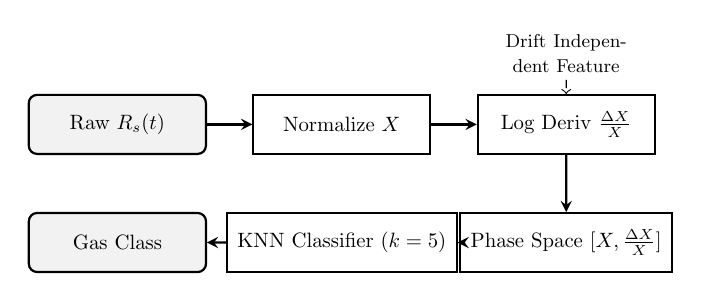
\begin{tikzpicture}[node distance=3.8cm, scale=0.75, transform shape]

% Defined styles
\tikzstyle{startstop} = [rectangle, rounded corners=3pt, minimum width=3cm, minimum height=1cm, inner sep=5pt, text centered, draw=black, thick, fill=gray!10]
\tikzstyle{process} = [rectangle, minimum width=3cm, minimum height=1cm, inner sep=5pt, text centered, draw=black, thick, fill=white]
\tikzstyle{arrow} = [thick,->,>=stealth]

% --- Row 1 (Left to Right) ---
\node (in1) [startstop] {Raw $R_s(t)$};
\node (pro1) [process, right of=in1] {Normalize $X$};
\node (pro2) [process, right of=pro1] {Log Deriv $\frac{\Delta X}{X}$};

% --- Row 2 (Right to Left) ---
% Position pro3 below pro2 to start the return path
\node (pro3) [process, below of=pro2, node distance=2cm] {Phase Space $[X, \frac{\Delta X}{X}]$};
\node (pro4) [process, left of=pro3] {KNN Classifier ($k=5$)};
\node (out1) [startstop, left of=pro4] {Gas Class};

% --- Arrows ---
\draw [arrow] (in1) -- (pro1);
\draw [arrow] (pro1) -- (pro2);
\draw [arrow] (pro2) -- (pro3); % Downward arrow
\draw [arrow] (pro3) -- (pro4);
\draw [arrow] (pro4) -- (out1);

% --- Label ---
% Placed above pro2 to save horizontal space
\node[text width=3cm, align=center, above of=pro2, node distance=1.2cm] (note1) {\small Drift Independent Feature};
\draw [dashed, ->] (note1) -- (pro2);

\end{tikzpicture}
\caption{System Architecture Pipeline. The data flows from left-to-right, then wraps around to the second row (snake layout) to conserve vertical space.}
\label{fig:pipeline}
\end{figure}

\subsection{Phase Space Trajectory Analysis}
The phase space representation effectively captures the dynamic behavior of the sensors. Fig. \ref{fig:mq3_phase} and Fig. \ref{fig:mq136_phase} illustrate the trajectories of the MQ-3 and MQ-136 sensors in the 2D plane defined by the Thermodynamic State ($X$) and the Kinetic State ($\dot{X}/X$).

\begin{figure}[htbp]
    \centering
    \begin{minipage}{0.48\textwidth}
        \centering
        \includegraphics[width=\linewidth]{fig_mq3_phase.jpg}
        \caption{MQ-3 Phase Space Trajectory. Note the tight clustering of 'No\_Gas' and the distinct loops for active gases.}
        \label{fig:mq3_phase}
    \end{minipage}\hfill
    \begin{minipage}{0.48\textwidth}
        \centering
        \includegraphics[width=\linewidth]{fig_mq136_phase.jpg}
        \caption{MQ-136 Phase Space Trajectory. The distinct shape compared to MQ-3 demonstrates the orthogonal sensitivity required for sensor fusion.}
        \label{fig:mq136_phase}
    \end{minipage}
\end{figure}

As observed, the Clean Air samples cluster tightly, representing a stable baseline. The active gas states (Butane and Smoke) and their corresponding recovery states form distinct loops. Notably, the topological structure differs between the two sensors; this variance provides the necessary orthogonality for the classifier.

\subsection{Classification Performance}
The system achieved an overall classification accuracy of 88.84\% on the test set. The performance for specific classes is detailed in the Confusion Matrix (Fig. \ref{fig:confusion}) and summarized below:

\begin{figure}[htbp]
    \centerline{\includegraphics[width=\linewidth]{fig_confusion.png}}
    \caption{Confusion Matrix (KNN, k=5). The matrix highlights the system's safety reliability (0 false negatives for 'No\_Gas') despite the chemical similarity between Butane and Smoke.}
    \label{fig:confusion}
\end{figure}

\begin{itemize}
    \item \textbf{Clean Air Robustness:} The system maintained 100\% precision and recall for No\_Gas, ensuring zero false alarms.
    \item \textbf{Smoke Detection:} Smoke was detected with high reliability (Precision: 84\%, Recall: 85\%).
    \item \textbf{Butane Sensitivity:} The classification of Butane presented a challenge (Recall: 63\%).
\end{itemize}

Confusion primarily occurred between Smoke and Butane (12 instances), indicating cross-sensitivity. However, confusion with `No\_Gas' was negligible, preserving the system's safety utility.

\subsection{Sensor Fusion Validation}
A comparative analysis highlights the necessity of the sensor array.
\begin{equation}
A_{MQ3} \approx 71.24\%, A_{MQ136} \approx 79.61\%, A_{Combined} \approx 88.84\%
\end{equation}
The combined array significantly outperforms individual sensors, validating the E-Nose approach.

% ==================================================================
% VII. CONCLUSION
% ==================================================================
\section{Conclusion}
This paper presented a robust Electronic Nose system built on the ESP32 platform, utilizing a novel phase-space trajectory mapping. By leveraging the normalized logarithmic derivative, we demonstrated that gas identity can be extracted as a topological invariant, decoupling the classification from baseline sensor drift. Experimental results confirmed that fusing data from MQ-3 and MQ-136 sensors resolves iso-resistive ambiguities, achieving 88.84\% accuracy and maintaining 100\% reliability in distinguishing clean air from contaminants.

% ==================================================================
% REFERENCES
% ==================================================================
\bibliographystyle{IEEEtran}
\begin{thebibliography}{00}

\bibitem{yan2015enose}
J. Yan \textit{et al.}, ``Electronic nose feature extraction methods: A review,'' \textit{Sensors}, vol. 15, no. 11, pp. 27804--27831, 2015.

\bibitem{yamazoe2009new}
N. Yamazoe and K. Shimanoe, ``New perspectives of gas sensor technology,'' \textit{Sensors and Actuators B: Chemical}, vol. 138, no. 1, pp. 100--107, 2009.

\bibitem{korotcenkov2012instability}
G. Korotcenkov and B. K. Cho, ``Instability of metal oxide gas sensors: Comparison of different approaches to drift compensation,'' \textit{Sensors and Actuators B: Chemical}, vol. 174, pp. 80--91, 2012.

\bibitem{siadat2014detection}
M. Siadat, E. Losson, D. Ahmadou, and M. Lumbreras, ``Detection Optimization Using a Transient Feature from a Metal Oxide Gas Sensor Array,'' \textit{Sensors \& Transducers}, vol. 171, no. 5, pp. 200--207, 2014.

\bibitem{gardner1991detection}
J. W. Gardner, ``Detection of vapours and odours from a multisensor array using pattern-recognition techniques,'' \textit{Sensors and Actuators B: Chemical}, vol. 4, no. 1-2, pp. 109--115, 1991.

\bibitem{pearce2003handbook}
T. C. Pearce, S. S. Schiffman, H. T. Nagle, and J. W. Gardner, \textit{Handbook of Machine Olfaction: Electronic Nose Technology}. Weinheim: Wiley-VCH, 2003.

\bibitem{atkins2018}
P. Atkins, J. de Paula, and J. Keeler, \textit{Atkins' Physical Chemistry}, 11th ed. Oxford: Oxford University Press, 2018.

\bibitem{cover1967nearest}
T. Cover and P. Hart, ``Nearest neighbor pattern classification,'' \textit{IEEE Transactions on Information Theory}, vol. 13, no. 1, pp. 21--27, 1967.

\end{thebibliography}

\end{document}
